\section{Smart meter privacy concerns}
The consumption data collected by a smart meter is fine-grained.
This fine-grained data means that it is easy to obtain knowledge about the consumer.
The following describes how one can obtain this knowledge and is based on \citet{privacy_memoir}.


An example setting which collected sixty days of power consumption from three homes consists of the following components:
\begin{itemize}
\item TED energy monitor
\item SheevaPlug
\end{itemize}
The TED energy monitor is connected to the two incoming electricty phases.
The SheevaPlug is connected to the router and the TED energy monitor and is used to access the data remotely.
The TED energy monitor returns a tuple $(t,p)$ where $t$ is the time and $p$ is the powerusage used since the last measurement.
The power is measured every second, so we have a tuple for every second with the time and the power used the past second.
At last the three households are supposed to make a power activity journal for a minimum of three days.
Which means to write down when they turn on and off any electric devices.

When the data is collected the data is analysed in four steps:
\begin{itemize}
\item Pre-process data
\item Tag power events
\item Filter out automated appliances
\item Map events to real life events
\end{itemize}

The data is pre-processed by using DBSCAN which is a density based clustering algorithm.
This helps group up power tuples into power segments, where a power segment is a collection of power tuples with a pattern adjacent in time.
Each power segment gets then tagged with a label, start time, average power, duration, beginning power step and a shape label.


On \cref{consumption_one_day} we are able to see the consumption data for one househole after two steps of analysis.
On the x-axis we have time in hours, midnight to midnight, on the y-axis we have power usage in kWh.
Already after two steps of analysis we are able to say something about when there is activity in the household.
We can also see how there are some automated appliances that are on all the time or at certain intervals.
We can determine this by assuming that there probably is almost no activity in te night and by collecting data over several days.


\begin{figure}
  \begin{center}
    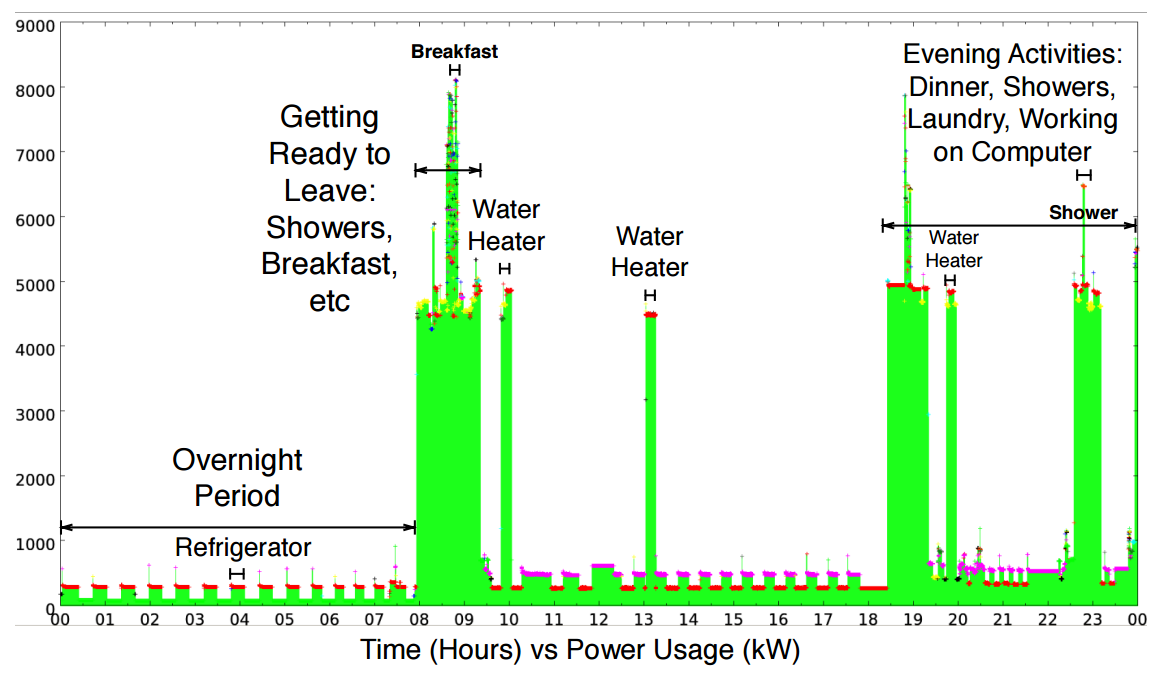
\includegraphics[width=\textheight, angle=90]{consumption_one_day.png}
  \end{center}
  \caption{A day of consumption data after two steps of analysis and with labels from real life events taken from the power activity journal.}
  \label{consumption_one_day}
\end{figure}


